%%%%%%%%%%%%%%%%%%%%%%%%%%%%%%%%%%%%%%%%%%%%%%%%%%%%%%%%%%%%
% preamble
%%%%%%%%%%%%%%%%%%%%%%%%%%%%%%%%%%%%%%%%%%%%%%%%%%%%%%%%%%%%
\documentclass{book}
\usepackage{ctex}
\usepackage{indentfirst} 
% code block
\usepackage{listings}
\usepackage{xcolor}
\lstset{ 
 breaklines,
 numbers=left,                                       
 numberstyle=\tiny\color{black},                   
 frame=none,                                          
 backgroundcolor=\color[RGB]{224,224,244},          
 keywordstyle=\color[RGB]{40,40,255},              
 numberstyle=\footnotesize\color{darkgray},           
 commentstyle=\it\color[RGB]{0,96,96},               
 stringstyle=\rmfamily\color[RGB]{128,0,0},   
 showstringspaces=false,                             
 language=Python,                               
}
% link
\usepackage[colorlinks,linkcolor=green]{hyperref}
\usepackage{graphicx} 
% 纸张设置
\usepackage{geometry}
\geometry{a4paper} % 纸张大小
\geometry{left=2cm} % 左边距
\geometry{right=2cm} % 右边距
\geometry{top=1cm} % 顶部边距
\geometry{bottom=0.5cm} % 底部边距
\geometry{hcentering}  % 水平居中
\geometry{vcentering} % 垂直居中

\begin{document}
\tableofcontents
%%%%%%%%%%%%%%%%%%%%%%%%%%%%%%%%%%%%%%%%%%%%%%%%%%%%%%%%%%%%
% 参考
%%%%%%%%%%%%%%%%%%%%%%%%%%%%%%%%%%%%%%%%%%%%%%%%%%%%%%%%%%%%
\chapter{参考}
\section{Course}
\noindent MOOC\\
\url{https://www.icourse163.org/course/ZJU-1003377027}\\
\url{https://www.icourse163.org/course/CUG-1003556007}\\
\url{https://www.icourse163.org/course/BIT-1001872001}\\
\url{https://www.icourse163.org/course/FJNU-1205696811}\\
\url{https://www.icourse163.org/course/ZJUT-1002694018}\\
David Silver(UCL)\\
\url{http://www0.cs.ucl.ac.uk/staff/D.Silver/web/Teaching.html}\\
Emma Brunskill(Stanford)\\
\url{https://onlinehub.stanford.edu/cs234}\\
Katerina\&Russ(CMU)\\
\url{https://katefvision.github.io/}\\
Sergey Levine(UC Berkeley)\\
\url{http://rail.eecs.berkeley.edu/deeprlcourse/}\\
李宏毅\\
\url{https://www.bilibili.com/video/av24724071?from=search&seid=8124301089510362159}\\
莫烦\\
\url{https://www.bilibili.com/video/av16921335}
\section{Book}
\noindent 郭宪\&方勇纯\\
《深入浅出强化学习:原理入门》\\
Richard S. Sutton and Andrew G. Barto\\
\url{http://www.incompleteideas.net/book/RLbook2018.pdf}\\
Code for Sutton's Book\\
\url{https://github.com/ShangtongZhang/reinforcement-learning-an-introduction}\\
Csaba Szepesvári\\
\url{https://sites.ualberta.ca/~szepesva/RLBook.html}
\section{Web}
\noindent \url{https://spinningup.openai.com/en/latest/index.html#}\\
\url{https://medium.com/@yuxili/resources-for-deep-reinforcement-learning-a5fdf2dc730f}\\
\url{https://zhuanlan.zhihu.com/sharerl}
\section{Environment}
\noindent \url{gym.openai.com}\\
\url{http://vizdoom.cs.put.edu.pl/}
\section{Other}
\noindent 大红豆与小薏米\\
\url{https://www.bilibili.com/video/av49055416}\\
\url{https://www.bilibili.com/video/av48758533}
%%%%%%%%%%%%%%%%%%%%%%%%%%%%%%%%%%%%%%%%%%%%%%%%%%%%%%%%%%%%
% 递归
%%%%%%%%%%%%%%%%%%%%%%%%%%%%%%%%%%%%%%%%%%%%%%%%%%%%%%%%%%%%
\chapter{递归}
\section{概念}
程序调用自身的编程技巧称为递归,递归问题的关键是写出递推关系式和边界条件,
递推关系式的左边是函数名,递归关系的右边是函数返回值,边界条件是函数的终
止条件。
\section{示例}
计算斐波那契数列的第n项:1,1,2,3,5,8,...
\begin{lstlisting} 
def fib(n): # 递归表达式的左边
    if n == 1: # 边界条件
        return 1
    elif n == 2: # 边界条件
        return 1
    else:
        return fib(n-1)+fib(n-2) # 递归表达式的右边
\end{lstlisting}   
\section{衍生}
计算斐波那契数列的前$n$项和
分析:如果知道前$n-1$项的和为$Sum(n-1)$,则$Sum(n)=fib(n)+Sum(n-1)$
\begin{lstlisting} 
# 计算fib(n)
def fib(n): 
    if n == 1: 
        return 1
    elif n == 2: 
        return 1
    else:
        return fib(n-1) + fib(n-2) 
# 计算Sum(n)
def Sum(n):
    if n == 1:
        return 1
    return fib(n) + Sum(n-1)
\end{lstlisting}   
%%%%%%%%%%%%%%%%%%%%%%%%%%%%%%%%%%%%%%%%%%%%%%%%%%%%%%%%%%%%
% 动态规划
%%%%%%%%%%%%%%%%%%%%%%%%%%%%%%%%%%%%%%%%%%%%%%%%%%%%%%%%%%%%
\chapter{动态规划}
\section{概念}
\noindent 重叠子问题\\
状态转移方程
\section{示例}
\begin{enumerate}
\item 斐波那契数列\\
给定一组斐波那契数列:1,1,2,3,5,8,...;其状态转移方程为:$F(n)=F(n-1) + F(n-2) (n>2)$
\begin{lstlisting}
memo = []
def fib(n):
    memo.append(1)
    memo.append(1)
    if n==1 or n==2:
        return 1
    elif n>2:
        for i in range(n-2):
            memo.append(memo[i] + memo[i+1]) 
        return memo[-1]
\end{lstlisting}
\item 最大工作报酬\\
\begin{figure}[!htbp]
\centering
\caption{最大工作报酬}
\includegraphics[width=6cm]{./res/最大工作报酬.pdf}
\end{figure}

如果只有1工作可选,则最大报酬为$dp(1)=5$\\
如果只有1,2两个工作可选,则最大报酬为$dp(2)=5$\\
如果可选工作为1,2,3则最大报酬为$dp(3)=8$\\
如果可选工作为1,2,3,4则最大报酬为$dp(4)=max(4+dp(1),dp(3))$\\
如果可选工作为1,2,3,4,5则最大报酬为$dp(5)=max(6+none, dp(4))$\\
如果可选工作为1,2,3,4,5,6则最大报酬为$dp(6)=max(3+dp(2), dp(5))$\\

\setlength{\parindent}{2em} 从i份工作可选过渡到i+1份工作可选的过程中,第i+1份工作如果做的话则报酬为第i+1份工作的报酬加上dp(最大可做工作的序号),如果第i+1份工作不做的话则最大报酬为dp(i);所以状态转移方程为:\\
dp(i+1)=max(第i+1份工作的报酬+dp(最大可做工作的序号),dp(i))

\item 最大不相邻元素子序列和
\begin{figure}[!htbp]
\caption{最大不相邻元素子序列和}
\includegraphics[width=6cm]{./res/最大子序列和.pdf}
\centering
\end{figure}

\noindent 如果只有第0号元素,dp(1)=1\\
如果只有第0,1号元素,dp(2)=2\\
如果只有第0,1,2号元素,dp(3)=max(arr[3]+dp(1),dp(2)\\

\setlength{\parindent}{2em} 从一个长为i的序列扩展到长为i+1的序列的状态转移方程为:\\
$$dp(i+1)=max(dp(i),dp(i-1)+arr[i+1])$$
\begin{lstlisting} 
def dp(arr):
    if len(arr)==1:
        return arr[0]
    if len(arr)==2:
        return max(arr[0], arr[1])
    if len(arr)>=3:
        sumMemo=[arr[0], max(arr[0], arr[1])]
        for i in range(2, len(arr)):
            n = max(sumMemo[i-1],sumMemo[i-2]+arr[i])
            sumMemo.append(n)
        return sumMemo[-1]
arr=[1,2,4,1,7,8,3]
dp(arr) # 15
\end{lstlisting}   
\item 定和组合\\
从arr=[3,34,4,12,5,2]组合出所有S=9的子序列\\
\begin{figure}[!htbp]
\caption{定和组合}
\includegraphics[width=14cm]{./res/定和组合.pdf}
\centering
\end{figure}

\begin{figure}[!htbp]
\begin{lstlisting}
import numpy as np 
def dp(arr, S): 
    memo = dict() 
    for i in range(len(arr)): 
        memo[i] = {'choose':[], 'not choose':[]} 
        present = arr[i] 
        if i == 0: 
            if S-present>0: 
                memo[i]['choose'].append(S-present) 
            memo[i]['not choose'].append(S) 
        else: 
            if memo[i-1]['choose']: 
                for j in memo[i-1]['choose']: 
                    if j-present==0: 
                        print('YES') 
                    if j-present>0: 
                        memo[i]['choose'].append(j-present) 
                    memo[i]['not choose'].append(j) 
            if memo[i-1]['not choose']: 
                for k in memo[i-1]['not choose']: 
                    if k-present==0: 
                        print('YES')  
                    if k-present>0: 
                        memo[i]['choose'].append(k-present)  
                    memo[i]['not choose'].append(k)   
    print(memo) 
arr=[3,34,4,12,5,2] 
dp(arr, 9)
\end{lstlisting} 
\end{figure}
\end{enumerate}
%%%%%%%%%%%%%%%%%%%%%%%%%%%%%%%%%%%%%%%%%%%%%%%%%%%%%%%%%%%%
% 强化学习
%%%%%%%%%%%%%%%%%%%%%%%%%%%%%%%%%%%%%%%%%%%%%%%%%%%%%%%%%%%%
\chapter{强化学习}
强化学习中agent通过和环境互动不断的试错(trial and error)来得到环境的
反馈,根据反馈来纠正自己的行动策略;具体来说,agent根据状态$S$来采取动作
$A$,得到环境返回的奖励$R$,和下一时刻的状态$S'$,不断的重复这一过程来
采集环境反馈回来的数据。\\
\section{马尔可夫过程}

\section{马尔可夫决策过程}
rrr
\section{强化学习的特点}
\begin{itemize}
	\item no supervisor
	\item not idd
	\item non-stationary
	\item reward is sparse and delayed
\end{itemize}
\section{分类}
\begin{enumerate}
\item 根据基于价值或者基于策略可分为:\\
Policy-based\\
Policy Gradient\\

Value-based\\
Q-learning\\
Sarsa\\

\item 根据环境是否已知分为:\\
Model-Based RL\\
Model-Free RL\\
MDP过程由一个五元组来确定<S, A, P, R, $\gamma$>,Policy是一个从S到
A的映射,R常常是已知的,所以环境是否已知是指状态转移矩阵P是否已知

\item 更新方式
单步更新
回合更新

\item 是否在线
on-policy
off-policy
\end{enumerate}
%%%%%%%%%%%%%%%%%%%%%%%%%%%%%%%%%%%%%%%%%%%%%%%%%%%%%%%%%%%%
% Value-based
%%%%%%%%%%%%%%%%%%%%%%%%%%%%%%%%%%%%%%%%%%%%%%%%%%%%%%%%%%%%
\chapter{Value-based}
\section{Q-learning}
\subsection{Paper}
\subsection{Code}
\subsection{收敛性证明}
%-----------------------------------------------------------
\section{Sarsa}
\subsection{Paper}
\subsection{Code}
%-----------------------------------------------------------
\section{DQN}
\url{https://www.youtube.com/watch?v=wrBUkpiRvCA}\\
\subsection{Paper}
\begin{figure}[!htbp]
\centering
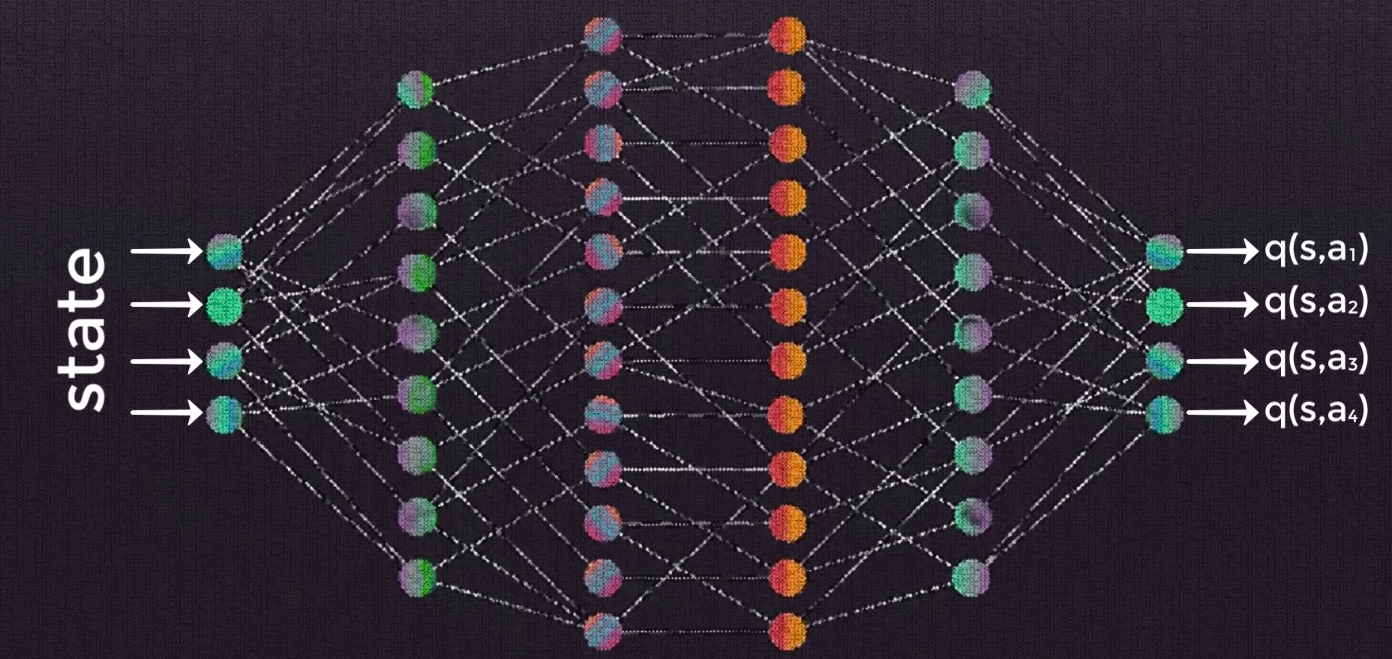
\includegraphics[width=6cm]{./res/DQN.jpg}
\caption{map state to action}
\end{figure}
\subsection{Code}

\subsection{衍生}
\subsubsection{Double DQN}
\subsubsection{Dueling Network}
\subsubsection{Prioritized Replay}
%%%%%%%%%%%%%%%%%%%%%%%%%%%%%%%%%%%%%%%%%%%%%%%%%%%%%%%%%%%%
% Policy-based
%%%%%%%%%%%%%%%%%%%%%%%%%%%%%%%%%%%%%%%%%%%%%%%%%%%%%%%%%%%%
\chapter{Policy-based}
\section{Policy Gradient}
\subsection{Paper}
\subsection{Code}
%-----------------------------------------------------------
\section{DPG}
\subsection{Paper}
\subsection{Code}
%-----------------------------------------------------------
\section{DDPG}
\subsection{Paper}
\subsection{Code}
%%%%%%%%%%%%%%%%%%%%%%%%%%%%%%%%%%%%%%%%%%%%%%%%%%%%%%%%%%%%
% Actor-Critic
%%%%%%%%%%%%%%%%%%%%%%%%%%%%%%%%%%%%%%%%%%%%%%%%%%%%%%%%%%%%
\chapter{Actor-Critic} 
AC\\
https://homes.cs.washington.edu/~todorov/courses/amath579/reading/PolicyGradient.pdf\\
A2C\\
https://openai.com/blog/baselines-acktr-a2c/\\
A3C\\
https://arxiv.org/abs/1602.01783
\section{AC}
\subsection{Paper}
\subsection{Code}
\begin{lstlisting}
import numpy as np
import tensorflow as tf
import gym
# tensorflow=1.14.0; gym=0.14.0; numpy=1.16.4 

# 超参数
OUTPUT_GRAPH = False
MAX_EPISODE = 3000
DISPLAY_REWARD_THRESHOLD = 200  # 刷新阈值
MAX_EP_STEPS = 1000             #最大迭代次数
RENDER = False  # 渲染开关
GAMMA = 0.9     # 衰变值
LR_A = 0.001    # Actor学习率
LR_C = 0.01     # Critic学习率

env = gym.make('CartPole-v0')
env.seed(1)  
env = env.unwrapped

N_F = env.observation_space.shape[0] # 状态空间
N_A = env.action_space.n             # 动作空间


class Actor(object):
    def __init__(self, sess, n_features, n_actions, lr=0.001):
        self.sess = sess

        self.s = tf.placeholder(tf.float32, [1, n_features], "state")
        self.a = tf.placeholder(tf.int32, None, "act")
        self.td_error = tf.placeholder(tf.float32, None, "td_error")  # TD_error

        with tf.variable_scope('Actor'):
            l1 = tf.layers.dense(
                inputs=self.s,
                units=20,    # number of hidden units
                activation=tf.nn.relu,
                kernel_initializer=tf.random_normal_initializer(0., .1),    # weights
                bias_initializer=tf.constant_initializer(0.1),  # biases
                name='l1'
            )

            self.acts_prob = tf.layers.dense(
                inputs=l1,
                units=n_actions,    # output units
                activation=tf.nn.softmax,   # get action probabilities
                kernel_initializer=tf.random_normal_initializer(0., .1),  # weights
                bias_initializer=tf.constant_initializer(0.1),  # biases
                name='acts_prob'
            )

        with tf.variable_scope('exp_v'):
            log_prob = tf.log(self.acts_prob[0, self.a])
            self.exp_v = tf.reduce_mean(log_prob * self.td_error)  # advantage (TD_error) guided loss

        with tf.variable_scope('train'):
            self.train_op = tf.train.AdamOptimizer(lr).minimize(-self.exp_v)  # minimize(-exp_v) = maximize(exp_v)

    def learn(self, s, a, td):
        s = s[np.newaxis, :]
        feed_dict = {self.s: s, self.a: a, self.td_error: td}
        _, exp_v = self.sess.run([self.train_op, self.exp_v], feed_dict)
        return exp_v

    def choose_action(self, s):
        s = s[np.newaxis, :]
        probs = self.sess.run(self.acts_prob, {self.s: s})   # 获取所有操作的概率
        return np.random.choice(np.arange(probs.shape[1]), p=probs.ravel())   # return a int


class Critic(object):
    def __init__(self, sess, n_features, lr=0.01):
        self.sess = sess

        self.s = tf.placeholder(tf.float32, [1, n_features], "state")
        self.v_ = tf.placeholder(tf.float32, [1, 1], "v_next")
        self.r = tf.placeholder(tf.float32, None, 'r')

        with tf.variable_scope('Critic'):
            l1 = tf.layers.dense(
                inputs=self.s,
                units=20,  # number of hidden units
                activation=tf.nn.relu,  # None
                # have to be linear to make sure the convergence of actor.
                # But linear approximator seems hardly learns the correct Q.
                kernel_initializer=tf.random_normal_initializer(0., .1),  # weights
                bias_initializer=tf.constant_initializer(0.1),  # biases
                name='l1'
            )

            self.v = tf.layers.dense(
                inputs=l1,
                units=1,  # output units
                activation=None,
                kernel_initializer=tf.random_normal_initializer(0., .1),  # weights
                bias_initializer=tf.constant_initializer(0.1),  # biases
                name='V'
            )

        with tf.variable_scope('squared_TD_error'):
            self.td_error = self.r + GAMMA * self.v_ - self.v
            self.loss = tf.square(self.td_error)    # TD_error = (r+gamma*V_next) - V_eval
        with tf.variable_scope('train'):
            self.train_op = tf.train.AdamOptimizer(lr).minimize(self.loss)

    def learn(self, s, r, s_):
        s, s_ = s[np.newaxis, :], s_[np.newaxis, :]

        v_ = self.sess.run(self.v, {self.s: s_})
        td_error, _ = self.sess.run([self.td_error, self.train_op],
                                          {self.s: s, self.v_: v_, self.r: r})
        return td_error
sess = tf.Session()
actor = Actor(sess, n_features=N_F, n_actions=N_A, lr=LR_A)  # 初始化Actor
critic = Critic(sess, n_features=N_F, lr=LR_C)     # 初始化Critic
sess.run(tf.global_variables_initializer())        # 初始化参数
if OUTPUT_GRAPH:
    tf.summary.FileWriter("logs/", sess.graph)        # 输出日志
# 开始迭代过程 对应伪代码部分
for i_episode in range(MAX_EPISODE):
    s = env.reset() # 环境初始化
    t = 0
    track_r = []    # 每回合的所有奖励
    while True:
        if RENDER: env.render()
        a = actor.choose_action(s)       # Actor选取动作
        s_, r, done, info = env.step(a)   # 环境反馈
        if done: r = -20    # 回合结束的惩罚
        track_r.append(r)  # 记录回报值r
        td_error = critic.learn(s, r, s_)  # Critic 学习
        actor.learn(s, a, td_error)        # Actor 学习
        s = s_
        t += 1

        if done or t >= MAX_EP_STEPS:
            # 回合结束, 打印回合累积奖励
            ep_rs_sum = sum(track_r)
            if 'running_reward' not in globals():
                running_reward = ep_rs_sum
            else:
                running_reward = running_reward * 0.95 + ep_rs_sum * 0.05
            if running_reward > DISPLAY_REWARD_THRESHOLD: RENDER = True  # rendering
            print("episode:", i_episode, "  reward:", int(running_reward))
            break
\end{lstlisting}
%-----------------------------------------------------------
\section{A2C}
\subsection{Paper}
\subsection{Code}
%-----------------------------------------------------------
\section{A3C}
\subsection{Paper}
\subsection{Code}
\end{document}